\chapter{Conversational Artificial Intelligence}
    Die hier beschriebenen Aspekte sind für das Untersuchungsdesign des Prototypen 
    in dieser Arbeit von Bedeutung. Aus diesem Grund werden zuerst die Differenzierungen
    der verschiedenen Begrifflichkeiten zum Themenbereich Chatbot aufgeführt (Kapitel \ref{DEFChatbot}). Anschließend folgt eine
    Ausführung des Natural Language Processings (Kapitel \ref{NLP}) und ein Einstieg in das Themengebiet des Maschinellen Lernens (Kapitel \ref{ML}), damit 
    ein Verständnis über die generelle Funktionsweise von Chatbots sowie ein Verständnis für 
    den Bedarf an Maschinellem Lernen erlangt wird. So können die Zusammenhänge im darauffolgenden Kapitel besser nachvollzogen werden. 
    Zum Schluss wird der aktuelle Stand der Forschung vorgestellt, um Bezüge und Abgrenzungen zu anderen Arbeiten aufzuzeigen (Kapitel \ref{StandderForschung}). 

    \section{Definitionen} \label{DEFChatbot}

        \subsection{Chatbot} \label{Chatbot}
        Chatbots, auch Chatterbots genannt, produzieren simulierte Gespräche, 
        in denen der menschliche Benutzer auf textbasierter natürlicher Sprache mit dem Chatbot interagiert.
        Chatbots haben ihren Ursprung in dem von Weizenbaum (1966) entwickelten ELIZA-System. \nocite{Weizenbaum.1966} \parencite[57 f.]{McTear.2016} \parencite[2 ff.]{Gnewuch.2017}

        \subsection{Conversational Agent}
        Conversational Agents (CA) können auf text- oder sprachbasierter natürlicher Sprache mit dem 
        Benutzer interagieren. Im Gegensatz dazu werden sprachbasierte CAs auch als virtuelle Assistenten bezeichnet, 
        die hauptsächlich auf gesprochene Eingaben reagieren. \parencite[51 f.]{McTear.2016} \parencite[3]{Gnewuch.2017}
        
        \subsection{Virtual Companion}
        Ein Agent, ein Chatbot oder ein virtueller Assistent, der möglichst viele von den folgenden Merkmalen enthält: 

        \begin{minipage}[t]{0.5\textwidth}
        \begin{itemize}
            \item eine kollaborative und freundliche langfristige Beziehung einhält
            \item ein angemessenes menschenähnliches Erscheinungsbild und Verhalten aufweist
            \item das Verständnis und die Akzeptanz des Benutzers erkennt\\
      \end{itemize}
        \end{minipage}
        \hfill
        \begin{minipage}[t]{0.5\textwidth}
            \begin{itemize}
            \item ein proaktives und wechselseitiges Verhalten darstellt
            \item Transparenz, Privatsphäre und Ethik beibehält
        \end{itemize}
    \end{minipage}
        wird als Virtual Companion bezeichnet. Er dient als vertrauenswürdiger Begleiter des Benutzers. \parencite[140]{strohmann.2021}
        Inwiefern der Prototyp ein Potenzial zum virtual Companion hat, wird in der Studie (vgl. Kapitel \ref{Kapitel5}) untersucht.

        Für die Beantwortung von RQ1 und RQ2 führt der Lernende zwei textbasierte Interaktion mit dem Prototypen durch. Daher wird im Folgenden der Begriff des Chatbots und des Conversational Agents verwendet.
        \section{Natural Language Processing } \label{NLP}
        Natural Language Processing (NLP) konzentriert sich auf die Interaktionen zwischen menschlicher Sprache und Computern. NLP 
        bietet eine Möglichkeit für Computer, die menschliche Sprache auf intelligente und nützliche Weise zu analysieren,
        zu verstehen und Bedeutungen abzuleiten. 
        Die Entwicklung von NLP-Anwendungen ist eine Herausforderung, da Computer traditionell vom Menschen verlangen,
        über eine Programmiersprache mit ihnen zu kommunizieren.
        Programmiersprachen sind präzise, eindeutig und hochstrukturiert.
        Im Gegensatz dazu ist die menschliche Sprache oft mehrdeutig und beinhaltet eine komplexe sprachliche Struktur.
        Um diesen Herausforderungen entgegenzuwirken, stellt NLP eine Computerlinguistik dar,
        welche mithilfe von Analysetechniken eine natürlich vorkommende und menschenähnliche Sprache im Computer abbildet 
        und ihren Generierungsprozess nachbildet. \parencite[42]{Sieber.2019}\parencite[2]{Liddy.2001} 
        
        Der Prototyp setzt verstärkt auf NLP, was sich aus dem \textbf{Natural Language Understanding (NLU)} und dem \textbf{Natural Language Generation (NLG)} zusammensetzt.
        Im nachfolgenden werden beide Bestandteile sowie das \textbf{Dialog Management System (DMS)} näher erläutert.
        \subsection{Natural Language Understanding} \label{NLU}
        Mit der natürlichen Sprache bitten Benutzer dem CA bestimmte Aufgaben auszuführen oder Informationen zu erfragen. 
        Intern verwendet ein CA dann NLU, um die gestellte Anfrage zu analysieren und auf die Anfrage des Benutzers zu reagieren.
        Das Hauptziel von NLU ist es beim Prozess der autonomen Gesprächsführung, strukturierte Daten aus unstrukturierten Spracheingaben des 
        Benutzers zu extrahieren. \parencite[2]{Ahmad.2021}\parencite[44]{Sieber.2019}
        NLU extrahiert Intents (dt. Absichten) und Entities (dt. Entitäten) aus Benutzeranfragen. Dabei stellen Intents 
        die semantisch-pragmatische Tiefenstruktur davon dar, was der Benutzer konkret beabsichtigt. Beispielsweise kann es sich dabei um die 
        Gesprächseröffnung, das Erfragen einer Information oder einer Bestellung handeln. Intents stellen eine große Anzahl an Realisierungsmöglichkeiten dar, welche
        sich zwischen Synonymen, Redensarten, Verben, Nominalstrukturen oder Hauptsätzen mit komplexen Nebensätzen unterscheiden können.
        Zum Beispiel kann anstatt der Äußerung: \glqq Wie wird das Wetter morgen in Braunschweig?\grqq{} auch folgendes gesagt werden: 
        \begin{itemize}
            \item \glqq Was sagt der Wetterbericht für Braunschweig?\grqq{}
            \item \glqq Brauche ich einen Schirm?\grqq{}
            \item \glqq Können wir heute Abend in Braunschweig grillen?\grqq{}
            \item \glqq Zeige das Wetter für den 12. April in Braunschweig.\grqq{}
        \end{itemize}
        Die unterschiedlichen Äußerungen, welche die gleiche Semantik aufweisen, sich aber in ihrer Pragmatik und Syntax unterscheiden, werden auch als \glqq Utterance\grqq{} bezeichnet.
        Auf den Intent \textit{ZeigWettervorhersage} können somit unterschiedlich viele
        Utterances verweisen. Je mehr Utterances der CA erkennen und zuordnen kann, desto besser zeichnet sich sein Sprachverständnis aus. 
        Entitäten stellen wichtige Informationen der Anfrage dar.
        Am Beispiel des Intents \glqq ZeigWettervorhersage\grqq{} muss näher bestimmt werden, für wann die Vorhersage 
        gelten soll und für welchen Ort (vgl. Abbildung \ref{fig:Utterance}). \parencite[138 f.]{Sieber.2019}
        \begin{figure}[H]
            \centering
            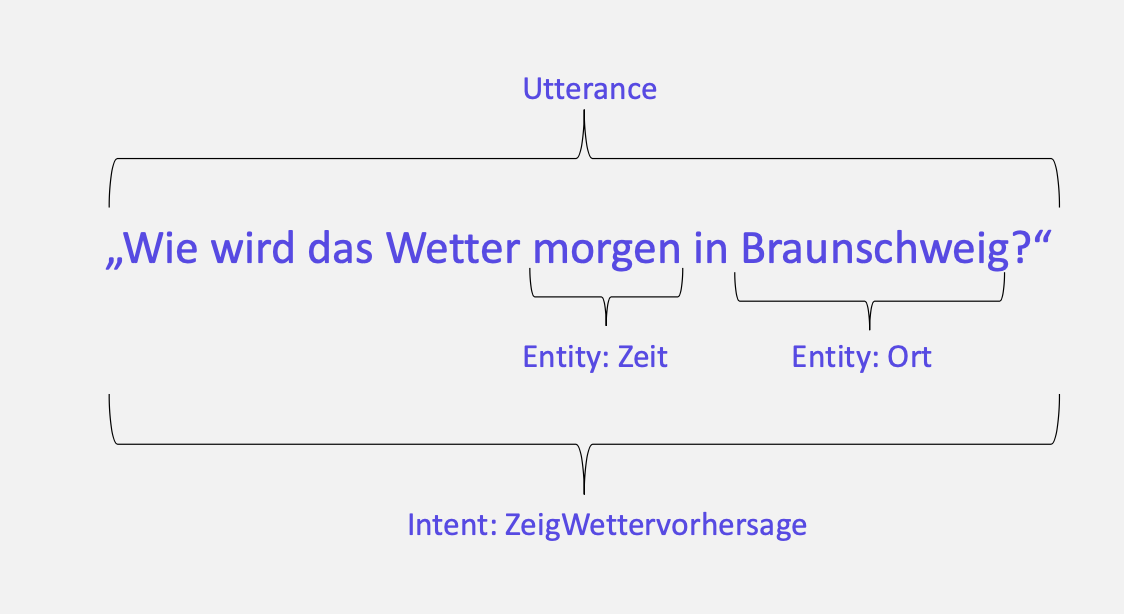
\includegraphics[width=0.6\linewidth]{images/utterance.png}
            \caption[Utterance, Entity, Intent]{Utterance, Entity, Intent (eigene Darstellung, in Anlehnung an \parencite[139]{Sieber.2019})}
            \label{fig:Utterance}
        \end{figure}
        
        Also muss der CA Entities wie \glqq morgen\grqq{}  oder \glqq heute Abend\grqq{} als Vorhersagezeit
        identifizieren, gleiches gilt für den Vorhersageort. 
        Für jeden benutzerdefinierten Intent muss die NLU mit einer Reihe von Anfragen trainiert
        werden, die verschiedene Möglichkeiten darstellen, wie ein Benutzer ein Intent ausdrücken könnte. \parencite[2]{Ahmad.2021}\parencite[138 f.]{Sieber.2019}
        Hier wird deutlich, dass die Formulierungen der Intents von den Benutzern frei gewählt werden können.
        Sobald der CA Pizza als Beispiel für Essen kennt, und der Benutzer nach Kuchen oder Salat fragt, sollte ein gutes NLU-System diese Benutzereingaben
        ebenfalls als Essen kennzeichnen können. \parencite[21]{Kong.2021}
        Dies stellt die Hauptverwendung von ML in Verbindung mit CAs dar, was in Kapitel \ref{ML} näher beschrieben wird.
        Während der Interaktion mit dem Prototypen werden Fragen aus dem ILS-Fragebogen gestellt.
        Der Prototyp muss die Antworten des Lernenden zum jeweiligen richtigen Intent zuordnen und
        Lernverhaltensmerkmale des Lernenden als Entities identifizieren. Diese 
        identifizierten Entities sind für die Lernstilidentifikation
        notwendig, wodurch RQ1 beantwortet werden kann. Der freie Formulierungsgrad spiegelt sich 
        darin wieder, dass die Lernenden auf die Fragen des ILS-Fragebogens unterschiedlich antworten können.

        Wenn eine NLU einen Intent falsch klassifiziert, versteht der CA die Anfrage nicht, was dazu führt, dass der CA auf eine ähnliche
        Anfrage antwortet oder die falsche Aufgabe ausführt.
        Eine falsche Klassifizierung von Entitäten führt hingegen dazu, dass der CA auf eine falsche Information antwortet.
        Um dem entgegenzuwirken, können Fallbacklösungen als Antwort des CAs implementiert werden, um dem Benutzer die Möglichkeit zu geben, 
        seine ursprüngliche Anfrage umzuformulieren. Dabei ist darauf zu achten, wann eine Fallbacklösung ausgelöst werden soll.
        Wird eine Fallbacklösung zu selten ausgeführt und der CA antwortet dadurch häufiger auf unklare Fragen (zu selbstbewusst),
        kann eine zu häufige Ausführung ein unsicheres Verhalten des CAs darstellen, was den Benutzer verärgert, da er die Frage häufig umformulieren muss.
        \parencite[3]{Ahmad.2021}\parencite[139]{Sieber.2019} 
        Aufgrund der geringen Trainingsdaten verwendet der Prototyp die Fallbacklösung.
        
        \subsection{Natural Language Generation}
        NLG wandelt die Antwort des CAs in Text um, der von dem Benutzer gelesen werden kann. 
        Es wird zwischen Template basierter und Deep Learning basierter Methode unterschieden, eine Antwort zu geben.
        Die Template basierte Methode basiert auf vereinfachten und von Menschen erstellten Antworten, welche wenig Flexibilität
        aufzeigen. Dennoch geben diese Antworten eine gute Lesbarkeit für die Menschen. Hingegen kann die Deep Learning basierte Methode flexible
        und personalisierte Antworten erzeugen. Die Antworten werden
        automatisch erstellt. Dadurch ist die Qualität und die Beständigkeit dieser Antworten schwer zu kontrollieren.
        In der Praxis wird oft zu der Template basierten Methode tendiert. 
        Um mehr Flexibilität gewährleisten zu können, wird eine Antwort zufällig aus einem Pool von Template basierten Antworten gewählt. \parencite[24]{Kong.2021}
        Aufgrund von wenigen Trainingsdatensätzen basiert der Prototyp der vorliegenden Arbeit auf einer Template basierten Methode als NLG.
        Die Entwicklung des Deep Learning Ansatzes als NLG kann in der Weiterentwicklung des Prototyps in Betracht gezogen werden. 
       
        \subsection{Dialog Management System} \label{DMS}
        Das DMS ist das Kontrollorgan der Mensch-Maschine Interaktion. Die Hauptaufgabe des DMS besteht darin, den gesamten 
        Unterhaltungsfluss zu koordinieren und zu managen. Durch die Analyse des Kontextes der Unterhaltung entscheidet das DMS, ob die zugrunde 
        liegenden Informationen zur Identifikation der Benutzerabsicht ausreichend sind, um eine entsprechende Aktion oder Datenbankanfrage auszuführen.
        Sobald das DMS nicht genügend Informationen für eine eindeutige Zuordnung der Benutzerabsicht hat, werden die Fallbacklösungen (vgl. Kapitel \ref{NLU})
        eingeleitet. 
        Neben der Steuerung des Ein- und Ausgabeprozesses enthält das DMS den Dialogverlauf. \parencite[23 f.]{Kong.2021} \parencite[59 f.]{Sieber.2019}
        Anhand des Dialogverlaufs können die identifizierten Intents und Entities nachvollzogen werden.
        Während des Dialogs zwischen Prototyp und Lernendem stellt der Prototyp Fragen aus dem ILS-Fragebogen. Die Antworten des Lernenden sollen gesammelt werden, da sie zur Lernstilklassifikation wichtig sind.
        Die 17 Fragen im Dialog werden mithilfe einer Form und Slots ausgeführt. Dies ermöglicht das Sammeln von Informationen des Lernenden. Des Weiteren bietet die Form mithilfe von Slots eine Möglichkeit, dass die einzelnen Fragen in einer gewissen Reihenfolge 
        gestellt werden können. \footnote{\url{ https://rasa.com/docs/rasa/2.x/forms}, aufgerufen am 26.01.2022} Der Slot stellt den Arbeitsspeicher des Bots dar. \footnote{\url{ https://rasa.com/docs/rasa/domain}, aufgerufen am 26.01.2022}  
        Die nächste Frage taucht erst auf, wenn die vorherige Frage beantwortet bzw. der Slot mit seiner zu erwartenden Entity gefüllt wurde.
        Anhand der Antworten des Lernenden zu den Fragen des ILS-Fragebogens können die identifizierten Intents, Entities sowie Slots analysiert werden.
        Mithilfe dieser Analyse kann die Klassifikation des Lernstils geprüft werden.
        
        Das Zusammenspiel der Komponenten NLU, DMS, NLG und Learner stellt das folgende Beispiel dar. Dabei bezieht sich das Beispiel auf eine Frage aus dem ILS-Fragebogen.
        \begin{itemize}
            \item[] \textit{DMS}: Activated Form: ILS-Questionnaire, next question: two
            \item[] \textit{NLG}: Do you tend to be realistic or innovative?
            \item[] \textbf{Learner: I think I tend to be more realistic}
            \item[] \textit{NLU Intent}: ILS-Question-two
            \item[] \textit{NLU Entity}: realistic
            \item[] \textit{DMS}: Activated Form: ILS-Questionnaire, Got Entity, Got Slot with Entity realistic, Slot filled, FS-Dimension-Score: sensor = sensor + 1, next question: three
            \item[] \textit{NLG}: Do you prefer the idea of certainty or hypothesis?
        \end{itemize}

\section{Maschinelles Lernen}\label{ML}
    Die Grundidee des Maschinellen Lernens ist, dass aus Beispielen Regelmä{\ss}igkeiten, Muster oder Modelle extrahiert bzw.
    gelernt werden und mit deren Hilfe neue Daten klassifiziert oder künftige Werte vorhergesagt werden können.
    KI-Systeme, die auf Maschinellem Lernen (ML) beruhen, werden mit diesen Beispielen bzw. Daten (Trainingsinstanzen)
    iterativ trainiert. Die Algorithmen\footnote{ Ein Algorithmus stellt aufeinanderfolgende Anweisungen dar, die ausgeführt werden, damit eine Eingabe in eine Ausgabe transformiert wird. Zum Beispiel kann ein Algorithmus konzipiert werden, der eine unsortierte Menge von Zahlen als Eingabe in eine geordnete Liste ausgibt. \parencite[2]{Alpaydin.2019}}
    des ML lernen aus diesen problemspezifischen Trainingsdaten.
    Sobald die Lernphase beendet ist, entstehen Modelle, welche allgemeine Regeln durch das Erkennen 
    von Mustern, Beziehungen und Regelmäßigkeiten in den Trainingsdaten bilden, um nun korrekte Entscheidungen bei
    unbekannten Daten treffen zu können.
    Der Lernprozess für die Erstellung eines ML-Modells kann in den Lernmodus und Aufgabentyp unterteilt werden. \parencite[35]{deru.2020}
        
        Für das Natural Language Processing werden die Supervised Learning (SL) Ansätze verwendet.
        Das SL Verfahren bildet ein mathematisches Modell ab, welches Datensätze mit Input und 
        dem zu erwartenden Output enthält, sodass dem System vorgegeben wird, was es lernen soll.
        Somit besteht jedes Trainingspaar aus der richtigen Antwort zu jeder Eingabe. Basierend auf diesen 
        Trainingspaaren wird das Modell gelernt, sodass für jede neue Eingabe das System die möglichst  
        korrekte Ausgabe gibt. \parencite[5]{Kong.2021}\parencite[39]{deru.2020}
    
        Der Prototyp dieser Arbeit nutzt unter anderem das SL, um aus unbekannten Benutzereingaben Entities für die Lernstilklassifikation zu extrahieren. 
        Dazu wird er mit einer Reihe von annotierten Texteingaben und 
        Beispielen versehen. Dadurch weiß der Prototyp, wonach er bei unbekannten Benutzeräußerungen 
        suchen soll und wie diese zu interpretieren sind.
           
        CAs beziehen sich auf den Aufgabentyp der Klassifikation.
        Die Aufgabe besteht darin, aus den Merkmalen der eingegebenen Benutzeräußerung
        eine dem Prototypen bekannte Klasse der Intents zu klassifizieren. \parencite[39]{deru.2020} \parencite[37 f.]{gentsch.2018}
        Zum Beispiel 
        soll durch die Benutzereingabe \glqq Hello\grqq{} die Intentklasse \glqq greet\grqq{}
        klassifiziert werden.

        Abschließend unterstützt das ML das NLP, indem die Eingabe des Dialogpartners nicht exakt den, in der Maschine hinterlegten Utterances, 
        entsprechen muss. Denn die Maschine soll die Absicht eines Nutzers ohne zugeordneter Erkennungsregel verstehen und dann antworten. \parencite[142]{Sieber.2019}
        Zum Beispiel soll der Prototyp den Intent \glqq whatDidYouDoYesterday\grqq{} auch bei Utterances wie 
        \glqq I was playing soccer with my friends\grqq{}  oder \glqq I was playing basketball with some students\grqq{} erkennen, sodass 
        unabhängig von der Sportart der Intent klassifiziert wird.
        Dadurch muss nicht jede mögliche Formulierung des Satzes eingegeben werden.
        Grundlage dieses Verhaltens sind Beispieldaten, mit denen die Maschine trainiert wurde. Anhand dieses Lernprozesses lernt 
        die Maschine mithilfe von Wahrscheinlichkeitsvergleichen eigenständig Muster in den Daten zu erkennen und diese der entsprechenden 
        Antwort zuzuordnen.\footnote{\url{ https://www.kiko.bot/blog/allgemein/maschinelles-lernen-bei-chatbots-chatbot-trainieren/}, aufgerufen am 04.01.2022}



    \section{Stand der Forschung} \label{StandderForschung}

    Für die vorliegende Arbeit wurden drei Forschungsarbeiten näher in Betracht gezogen, um RQ1 und RQ2 beantworten zu können.
    Die nachfolgende Abbildung \ref{fig:forschung} skizziert diese.
 
    \begin{figure}[H]
        \centering
        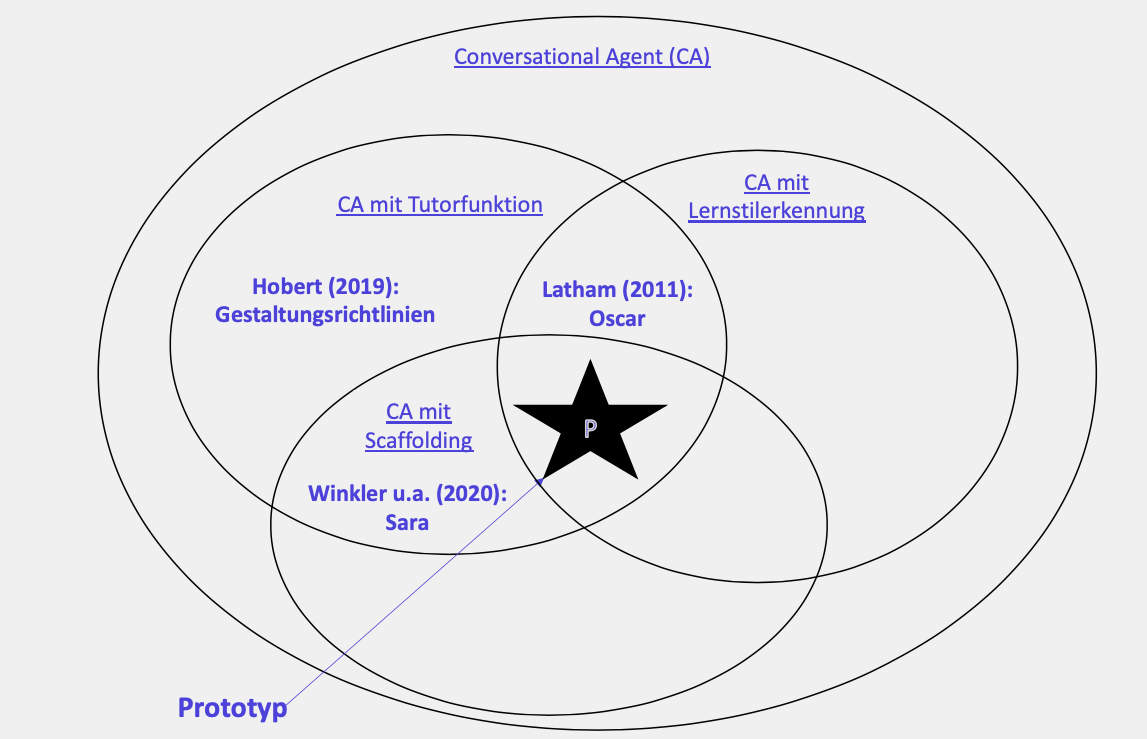
\includegraphics[width=0.9\linewidth]{images/forschung.png}
        \caption[Stand der Forschung]{Stand der Forschung (eigene Darstellung)}
        \label{fig:forschung}
    \end{figure}
    
    In der Literatur kennzeichnet die Hauptaufgabe eines CAs im Education-Bereich die Unterstützung des Lehrbetriebs.
    Hobert (2019) skizziert Gestaltungsrichtlinien zu einem Chatbot basierten Lernsystem, das
    Programmieranfängern beim Lösen von Programmieraufgaben unterstützt, 
    sobald kein menschlicher Lehrassistent verfügbar ist (z.B. am Wochenende).
    Durch diese individuelle Betreuung können Dozenten entlastet werden, sodass
    Programmierkurse auch bei stark steigenden Studierendenzahlen
    durchgeführt werden können. Des Weiteren können die
    meisten Fragen möglicherweise automatisch beantwortet werden, sodass  
    menschliche Lehrassistenten sich auf die Beantwortung der verbleibenden
    schwierigeren Fragen konzentrieren können. \parencite[5 ff.]{Hobert2019SayHT}
    Nach der ersten Designiteration des 
    Coding Tutors wurden Feedbackbögen zu den ersten Skizzen gesammelt.
    Es wurden Studierende in einem Java Anfängerkurs des 
    Studiengangs Wirtschaftsinformatik befragt. Ein auffallender Kommentar war, 
    dass die Befürchtung bestand, dass die \glqq Schritt-für-Schritt-Anleitung\grqq{} den Lerneffekt
    mindern würde, wenn zu viel Anleitung gegeben wird. \parencite[10]{Hobert2019SayHT}
    Der Prototyp der vorliegenden Arbeit gibt beim Quiz-Spiel Hilfestellung zum Lösen der Quiz-Fragen. 
    Dabei wird beachtet, nicht zu viel von der Lösung bei der Hilfestellung zu verraten, sodass 
    der Lernende durch eigene kognitive Anstrengung zur Lösung kommen muss.
        
        Inwiefern CAs den Lehrbetrieb unterstützen können, haben Winkler u.a. (2020) gezeigt und einen CA namens Sara entwickelt, der während einer 
        Online-Vorlesung erscheint. 
        Sara unterbricht den Videovortrag nach jedem Unterkapitel
        und stellt jedem Lernenden eine Reihe von Verständnisfragen, um den gerade gesehenen und gehörten Inhalt zu wiederholen.
        Dabei können die Lernenden mit Sara per Text oder Stimme interagieren.
        Bei einer richtigen Antwort fährt Sara mit der nächsten Frage fort. 
        Wenn Sara eine falsche Antwort erkennt, oder der Lernende nicht weiß,
        wie er antworten soll, öffnet sich ein weiteres Dialogfenster für Erklärungen und Fragen 
        des Lernenden. Nach der Erklärung wird die Frage erneut gestellt, und die Lernenden haben noch einmal die Möglichkeit, 
        die Frage erneut zu beantworten, bevor die Antwort erklärt wird und Sara mit der nächsten Frage fortfährt. \parencite[4 f.]{winkler_hobert_salovaara_söllner_leimeister_2020}
        Mit diesem Mechanismus versucht Sara, das scaffolding Verhalten von Pädagogen in der Interaktion mit ihren Lernenden zu imitieren. 
        Das scaffolding Verhalten von Pädagogen bezeichnet eine Unterstützung des Lernprozesses durch die Bereitstellung einer ersten Orientierungsgrundlage
        in From von Anleitungen oder Denkanstößen. \footnote{\url{https://lexikon.stangl.eu/13399/scaffolding}, aufgerufen am 18.11.2021}
        Der Prototyp dieser Arbeit greift beim Quiz-Spiel auf das Scaffolding Verhalten zurück. Bei einigen 
        Quiz-Fragen werden dem Lernendem  
        Hilfsfragen gegeben, um auf die richtige Lösung zu kommen.
        Die Ergebnisse der Studie zeigen einen positiven Effekt auf die Verwendung eines scaffolding textbasierten CA.
        Lernende, welche mit einem scaffolding textbasierten CA im Lernprozess interagiert haben, haben im Vortest zu der Programmiersprache Python ohne 
        einen scaffolding CA
        39.8 Punkte von 100 Punkten und im Nachtest mit einem scaffolding CA 73,1 Punkte von 100 Punkten erreicht. \parencite[8 f.]{winkler_hobert_salovaara_söllner_leimeister_2020}

        Latham u.a. (2010) haben ein conversational intelligent tutoring system (CITS)  namens Oscar entwickelt, der während eines Nachhilfegesprächs den Lernstil des Lernenden bestimmt und dann sein Lehrformat
        an den identifizierten Lernstil des Lernenden anpasst.
        Ein  intelligentes conversational Tutoringsystem sind Computerlernsysteme, die ihre Lerninhalte für eine Person personalisieren und über eine 
        natürliche Sprachschnittstelle zur Kommunikation per Text oder Sprache verfügen.
        Oscar klassifiziert den Lernstil nach dem Lernstilmodell 
        von Felder und Silverman (1988). Dafür nutzt Oscar den ILS-Fragebogen von Felder und Soloman (1991) (vgl. Kapitel \ref{ATL}).
        Oscar zielt darauf ab, einen menschlichen Tutor nachzuahmen, 
        indem er eine dialogorientierte Problemlösungsunterstützung im Bereich der 
        Datenbank Structured Query Language (SQL) anbietet.
        Zur Unterstützung des Nachhilfegesprächs können Diagramme, Bilder und interaktive Filme angezeigt werden. Aspekte des Verhaltens 
        und des Verständnisses des Lernenden fließen in die dynamische Einschätzung
        des Lernstils ein und ermöglichen es, den Unterrichtsstil so zu personalisieren, dass er am besten zu dem Schüler passt.
        \parencite[4]{Oscar}

        Der ILS-Fragebogen enthält 44 Fragen. Es wurde eine Pilotstudie mit 103 ausgefüllten ILS-Fragebögen durchgeführt,
        um zu untersuchen, welche Fragen die aussagekräftigsten waren, um den Lernstil zu bestimmen. 
        Die Studie ergab, dass 17 Fragen den gesamten Lernstil zu mindestens 75 \% vorhersagen können. 
        Sobald eine begrenzte Anzahl von ILS-Fragen in einen CITS zur Vorhersage des individuellen Lernstils des Lernenden 
        einbezogen werden, ist es am besten, diejenigen Fragen auszuwählen, die den allgemeinen Lernstil am genauesten vorhersagen.
        Für die Beurteilung des allgemeinen Lernstils als auch für dessen Stärke werden alle Fragen des ILS-Instruments benötigt.
        Allerdings sobald das Ausfüllen des ILS-Fragebogens
        durch eine implizite Vorhersage des Lernstils ersetzt wird, so ergibt sich aus den Studienergebnissen ein Ausgangspunkt für die Fragen, die am besten 
        den allgemeinen Lernstil bestimmen können. \parencite[51 f.]{Latham.2011}
        
        Das FS-Modell wurde für die Klassifizierung des Lernstils von Ingenieurstudenten entwickelt.
        In einer weiteren Pilotstudie mit 10 Teilnehmern wurde Oscar auf zwei Arten beurteilt.
        Sowohl wurde die Einschätzung des Lernstils durch Oscar bewertet als auch die Art und Weise, wie Oscar von dem Benutzer 
        während der Interaktion wahrgenommen wurde.
        Während des Tutor-Gesprächs werden die Lernstilwerte in Abhängigkeit vom Gespräch des Lernenden erhöht.
        Am Ende der Tutoring-Sitzung werden die Wertepaare jeder FS-Dimension verglichen, um die allgemeine Lernstiltendenz 
        des Schülers für diese Dimension (d.h. der höhere Wert) anzuzeigen. Die Werte des Lernstils hängen von der individuellen
        Tutorial-Sitzung einer Person ab. Sobald eine Kategorie nicht eindeutig bestimmt werden konnte, die einer bestimmten FS-Dimension nahelag,
        bleibt dieser Lernstil unklassifiziert. 
        Bei der Studie wurden drei Experimente durchgeführt.
        Experiment eins untersuchte die Art und Weise, wie der Lernende mit dem Lernmaterial und mit der Hilfestellungen von Oscar umging.  
        Experiment zwei untersuchte die Anzahl der Interaktionen mit Oscar während des Tutorials.
        Für das zweite Experiment wurde die Anzahl der Interaktionen während der Tutoring-Sitzung gezählt. 
        Die Hypothese lautete: \glqq Je diskursiver ein Schüler 
        ist (d. h. je mehr Interaktionen), desto mehr neigen sie zum verbalen Lernstil\grqq{}.
        Für Experiment drei wurde die 
        durchschnittliche Zeit zum Lesen von zehn Oscar-Wörtern für jeden Schüler berechnet.
        Die Hypothese war, dass \glqq je länger ein Schüler braucht, um Anweisungen zu lesen 
        (d. h. je weniger er mit Wörtern vertraut ist), desto mehr tendieren sie zum visuellen Lernstil\grqq{}. 
        Für die Studie wurden Studierende der Ingenieurswissenschaft ausgewählt, welche einen Pre-Test im Bereich SQL absolviert haben sowie den ILS-Fragebogen ausgefüllt haben.
        Nach dem Gespräch mit Oscar haben die Lernenden einen Post-Test durchgeführt. Der identifizierte Lernstil von Oscar 
        wurde mit dem Lernstil aus dem Fragebogen verglichen.
        Die Ergebnisse der ersten Pilotstudie sind vielversprechend, da in drei Fällen die Genauigkeit der Schätzung des Lernstils bei 70 \% lag und im schlechtesten Fall bei 50 \%.
        Darüber hinaus haben sich die 
        Testergebnisse zwischen Pre- und Post-Test um ca. 21 \% verbessert. Dennoch kann mit dieser kleinen Ausgangsstichprobe keine 
        eindeutige Schlussfolgerungen gezogen werden, daher bedarf es an einer weiteren Studie mit einer größeren Stichprobengruppe. \parencite[6 f.]{Oscar}

        Eine weitere Studie zu Oscar wurde mit 65 Lernenden durchgeführt, die bereits Erfahrung mit einem Bachelor-SQL-Kurs hatten. 
        Dabei wurden zu den drei bestehenden Experimenten noch zwei weitere hinzugefügt. Ferner wurde zusätzlich noch der Stil der 
        Tutorialfragen untersucht, bei denen die Teilnehmer die richtige Antwort gaben.
        Es wurde die Anzahl der richtigen theoretischen und der richtigen praktischen Fragen gezählt.
        Oscar hat den Lernstil als aktiv und sensorisch bei den Lernenden eingestuft, die in theoretischen Fragen bessere Leistungen zeigten. Bei 
        schlechterer Leistung in theoretischen Fragen
        wurden die Lernenden als reflektierend und intuitiv klassifiziert.
        Des Weiteren wurde eine Tutorial-Frage als eine allgemeine \glqq Trick-Frage\grqq{} gestellt, bei
        der die Antwort im erläuternden Text stand. Dadurch wurde die Detailgenauigkeit und Lesefähigkeit des Lernenden getestet. 
        Lernende, welche die Frage nicht richtig beantworteten, wurden als visuelle und intuitive Lerner bestimmt, während diejenigen,
        die richtig antworteten, als verbale und sensorische Lerner eingestuft wurden.
        Die experimentellen Ergebnisse zeigen, dass es möglich ist, einen Lernstil aus einem wechselseitigen Nachhilfegespräch
        in natürlicher Sprache vorherzusagen. Oscar hat alle Lernstile mit einer Genauigkeit zwischen 61-100 \% 
        im Rahmen des Index of Learning Styles erfolgreich klassifiziert.  \parencite[105 ff.]{Latham.2012}
        
        Der Prototyp dieser Arbeit verwendet in seinem Dialog zur Lernstilidentifikation des Lernenden 
        die 17 reduzierten Fragen des ILS-Fragebogens von Latham (2011). Allerdings findet die Klassifikation 
        des Lernstils, nicht während eines Nachhilfegesprächs statt, sondern in einem freundlichen Dialog.
        Dem Lernenden wird der identifizierte Lernstil am Ende des Dialogs mitgeteilt, sodass er sein 
        Lernverhalten diesem anpassen kann. Des Weiteren wendet sich der Prototyp im Gegensatz zu Oscar an allgemein Lernende, unabhängig vom 
        Studiengang. Zusätzlich bestimmt der Prototyp den Lernstil ein weiteres Mal in einer zweiten Interaktion zwischen 
        Lernendem und Prototypen. In einem Quiz-Spiel wird durch die angebotenen Hilfestellungen versucht, den Lernstil 
        des Lernenden zu identifizieren. Dabei wird sich an die Vorgehensweise von Oscars Hilfestellungen und Quiz-Fragen (Experiment 1, 4 und 5) während 
        seines Nachhilfegesprächs zu SQL orientiert. 

        An dieser Stelle soll noch einmal zu der aufgeführten Abbildung \ref{fig:forschung} Bezug genommen werden.
        Der Prototyp adaptiert von allen drei vorgestellten Forschungsansätzen einige Aspekte. Deshalb 
        findet er in der Abbildung dort seinen Platz, wo sich alle Kreise überschneiden. 

    \textbf{Kapitelzusammenfassung} 
    \begin{itemize}
        \item Conversational Agents können auf text- oder sprachbasierter natürlicher Sprache mit dem Benutzer interagieren. Dabei werden textbasierte Conversational Agents oft als Chatbots bezeichnet, mit denen über Textnachrichten interagiert wird. Für die Beantwortung von RQ1 und RQ2 führt der Lernende zwei textbasierte Interaktion mit dem Prototypen durch.
        \item Ein Virtual Companion dient als vertrauenswürdiger Begleiter des Benutzers.
        \item Der Einstieg ins NLP und ML wurde gegeben, um ein Verständnis für die Computerlinguistik zwischen Mensch und Maschine zu bekommen.
        \item NLP bietet eine Möglichkeit für Computer, die menschliche Sprache auf intelligente und nützliche Weise zu analysieren, zu verstehen und Bedeutungen abzuleiten.
        NLP setzt sich aus NLU und NLG zusammen.
        \item Das Hauptziel von NLU besteht darin: beim Prozess der autonomen Gesprächsführung, strukturierte Daten aus unstrukturierten Spracheingaben des Benutzers zu extrahieren.
        Somit extrahiert die NLU Intents und Entities aus Benutzeranfragen.
        Dabei stellen Intents die Benutzerabsicht, Entities die wichtigen Informationen aus der Anfrage und die Utterances die unterschiedlichen Benutzeräußerungen dar.
        \item Der Prototyp muss die Antworten des Lernenden zum richtigen Intent zuordnen und Lernverhaltensmerkmale des Lernenden als Entities identifizieren. Diese identifizierten Entities sind für die Lernstilidentifikation notwendig, wodurch RQ1 beantwortet werden kann.
        \item NLG wandelt die Antwort des CAs in Text um, der von dem Benutzer gelesen werden kann.
        \item Das DMS ist das Kontrollorgan der Mensch-Maschine Interaktion. Die Hauptaufgabe des DMS besteht darin, den gesamten Unterhaltungsfluss zu koordinieren und zu managen. Die 17 Fragen des ILS-Fragebogens werden im Dialog  mithilfe einer Form und Slots ausgeführt. Dies ermöglicht das Sammeln von Lernstilmerkmalen des Lernenden, wodurch die Lernstilklassifikation möglich wird. 
        \item Das ML unterstützt das NLP, indem die Eingabe des Dialogpartners nicht exakt den, in der Maschine hinterlegten Utterances, entsprechen muss. Die Maschine soll die Absicht eines Nutzers ohne zugeordneter Erkennungsregel verstehen und antworten können. Dadurch können die Lernenden auf die Fragen des ILS-Fragebogens unterschiedlich antworten. Des Weiteren wird das Extrahieren von Entities für die Lernstilklassifikation ermöglicht.
        \item Ein Bezug zu anderen Arbeiten sowie deren Abgrenzung wurde mithilfe des aktuellen Forschungsstandes aufgezeigt.
        Die gewonnenen Erkenntnisse, wie zum Beispiel das Scaffolding-Verhalten und die 17 reduzierten ILS-Fragen,
        wurden bei der Implementierung des Prototyps berücksichtigt, welche 
        im nachfolgenden Kapitel bei der Vorstellung des Prototyps näher aufgezeigt werden. 
    \end{itemize}